%%%%%%%%%%%%%%%%%%%%%%%%%%%%%%%%%%%%%%%%%%%%%%%%%%%%%%%%%%%%%%%
%
%\title{BioJS InterMine Table}
%
% A paper for the BioJS project on the BioJS.InterMine.Table
% component.
%
%%%%%%%%%%%%%%%%%%%%%%%%%%%%%%%%%%%%%%%%%%%%%%%%%%%%%%%%%%%%%%%

\documentclass[10pt,a4paper,twocolumn]{article}
\usepackage{f1000_styles}
\usepackage{listings}
\usepackage{hyperref}

\definecolor{dkgreen}{rgb}{0,0.6,0}
\definecolor{gray}{rgb}{0.5,0.5,0.5}
\definecolor{mauve}{rgb}{0.58,0,0.82}

\lstdefinelanguage{JavaScript}{
  keywords={typeof, new, true, false, catch, function, return, null, catch, switch, var, if, in, while, do, else, case, break},
  keywordstyle=\color{blue}\bfseries,
  ndkeywords={class, export, boolean, throw, implements, import, this},
  ndkeywordstyle=\color{darkgray}\bfseries,
  identifierstyle=\color{black},
  sensitive=false,
  comment=[l]{//},
  morecomment=[s]{/*}{*/},
  commentstyle=\color{purple}\ttfamily,
  stringstyle=\color{red}\ttfamily,
  morestring=[b]',
  morestring=[b]"
}

\lstset{
  frame=none,
  language=JavaScript,
  aboveskip=3mm,
  belowskip=3mm,
  showstringspaces=false,
  columns=flexible,
  basicstyle={\small\ttfamily},
  numbers=none,
  numberstyle=\tiny\color{gray},
  keywordstyle=\color{blue},
  commentstyle=\color{dkgreen},
  stringstyle=\color{mauve},
  breaklines=true,
  breakatwhitespace=true
  tabsize=3
}

\begin{document}

\title{\textit{BioJS} InterMineTable component:
A BioJS component for displaying data from InterMine compatible web-service endpoints.
}

\author[1]{Alexis Kalderimis \thanks{alex@intermine.org}}
\author[1]{Radek Štěpán \thanks{radek@intermine.org}}
\author[1]{Julie Sullivan \thanks{julie@flymine.org}}
\author[1]{Rachel Lyne \thanks{rachel@flymine.org}}
\author[1]{Michael Lyne \thanks{mike@intermine.org}}
\author[1]{Gos Micklem \thanks{g.micklem@gen.cam.ac.uk - corresponding author}}
\affil[1]{
    Department of Genetics and Cambridge Systems Biology Centre,
    Cambridge University, Downing Street, Cambridge, CB2 3EH, UK.
}

\maketitle
\thispagestyle{fancy}

\begin{abstract}

\textbf{Summary:}
The InterMineTable component is a reusable JavaScript
component as part of the BioJS project. It enables users to embed
powerful table-based query facilities in their websites with
access to genomic data-warehouses such as http://www.flymine.org,
which allow users to perform flexible queries over a wide range
of integrated data types.

\textbf{Availability:}
\url{http://github.com/alexkalderimis/im-tables-biojs} and
\url{http://github.com/biojs/biojs}

\textbf{Contact:} g.micklem@cam.ac.uk

\end{abstract}
\clearpage

\section*{Introduction}

There are currently a number of genomics data-warehouses available which are
powered by the InterMine ~\cite{smith2012} platform. This set includes large
curated services dedicated to the primary Model Organism database (MOD)
communities as part of the InterMOD project~\cite{sullivan2013}, the collected
data sets of research projects such as the modENCODE
project~\cite{contrino2012}, as well as a range of other resources including
metabolicMine~\cite{metabolicmine}, TargetMine~\cite{targetmine},
FlyTFMine~\cite{flytfmine}, and MitoMiner~\cite{mitominer}.  In addition to
being accessible through web-interfaces these resources also provide web-service
access (to be described in a forthcoming paper).

The InterMine system provides users with a number of benefits. A typical
InterMine instance, such as FlyMine~\cite{flymine} or
YeastMine~\cite{yeastmine}, contains feature annotations, protein data,
publications, biochemical pathways, orthology, Gene Ontology (GO), array
expression results, and other kinds of data, all integrated into a single
knowledge graph. This means end users are able to ask questions across different
data types. InterMine's particular data integration strategy puts minimal
limitations on the kinds of queries that can be performed: any arbitrary number
of data-sets can be referred to in the same query (provided links exist between
them) and a wide variety of logical contraints can be added. The InterMine
platform thus provides a basis for very flexible, user-defined
queries over linked data sets. 

The BioJS ~\cite{biojs} project seeks to provide a suite of reusable JavaScript
components that members of the bioinformatics community will find useful for
producing analysis and visualisation tools. The InterMineTable BioJS component
contributes towards this aim by adding a data query and exploration tool to the
set of BioJS components which exposes the full flexibility and power of user
defined queries over integrated linked data in a clear user interface.

\subsection*{Installation}

As a visual BioJS component, the intended audience is web-developers aiming to
provide extended functionality to web-based resources for life-scientists. It is
expected to be deployed within modern browser environments with access to
third-party resources. With this in mind, installation comprises of including
the dependencies for the InterMine table component on the page (usually added in
the head section of an HTML page), see Supplementary materials~\ref{sec:deps}. Once the
dependency on the InterMine tables library is loaded, the InterMineTable BioJS
component may be included (see code listing~\ref{code:loading}).

\begin{lstlisting}[caption={Loading the BioJS InterMine Table library}, label={code:loading}]
<script src="Biojs.InterMine.Table.js"></script>
\end{lstlisting}

This last resource contains the definition of the InterMine.Table BioJS
component. As it is not available from a reliable third party source, it
currently needs to be downloaded from the BioJS
registry~\cite{site:biojs-registry}, and hosted locally.

\subsection*{Usage}

This component is used by instantiating the InterMine table component in a
user-included JavaScript file, passing in the appropriate configuration for the
desired source of data as well as the query over those data.

Once instantiated, the results of the query against the specified integrated
data-warehouse are loaded into a component where they can be browsed and
manipulated.  This means that the two critical concepts for using this component
are 1) the location of the data-store, defined as the uniform resource locator
(URL) pointing at the root of a set of web-services, and 2) the query to be run
on the data in the store, defined in a configuration object. For example, to
load a table of data from FlyMine the user would want the URL to point to
FlyMine's webservices:

\begin{lstlisting}[caption={Specifying the Data-Store}, label={code:set-url}]
var url = "http://www.flymine.org/query";
\end{lstlisting}

The query can be broadly defined as a list of fields, identified by paths from a
root, constrained by a (possibly empty) set of filters. There are some
refinements to this (such as sort-order, optional element definition, and
constraint composition) for which more detailed documentation~\cite{site:pqdocs}
exists. The concept of a path is important to the idea of a graph of linked
data, as it enables chains of relationships between entities to be followed,
with minimal syntactic overhead. For example the chain of relationships
\emph{the names of the protein domains of the proteins encoded by the genes
belonging to a biochemical pathway} can be referred to as
\texttt{Pathway.genes.proteins.proteinDomains.name}.

A query is defined as a plain JavaScript object which can be simple, such as the 
following query, which requests the common name, scientific name and
taxon ID for all organisms in the data-store:

\begin{lstlisting}[
    caption={A simple Query, see Figure ~\ref{fig:1}},
    label={code:simple-query}]
// Available organisms
var query = {
  name: "An optional name",
  from: "Organism",
  select: ["commonName", "name", "taxonId"],
};
\end{lstlisting}

or arbitrarily complex, such as the following query which combines information
from multiple data sources (OMIM~\cite{omim}, PANTHER~\cite{panther},
Treefam~\cite{treefam}, KEGG~\cite{kegg}, Reactome~\cite{reactome},
FlyBase~\cite{flybase}) and across different organisms to find the
\textit{Drosophila melanogaster} genes in the pathways of genes which are
orthologous to human genes implicated in Alzheimer's disease:

\begin{lstlisting}[
    caption={A Complex Query, see Figure ~\ref{fig:complex}},
    label={code:complex-query}]
var disease = {
  from: "Disease",
  select: [
    "genes.homologues.homologue.pathways.genes.*"
  ],
  where: {
    "name": "Alzheimer*",
    "genes.organism.name": "Homo sapiens",
    "genes.homologues.homologue.organism.name": "Drosophila melanogaster"
  }
};
\end{lstlisting}

An element also needs to be present on the page where the table should be
loaded. This can be any element (although a \texttt{DIV} element is
conventional), and should be uniquely identifiable (through its ID for
instance).

\begin{lstlisting}[caption={Defining the Target Element}, label={code:target-el}]
var target = "#table-container";
\end{lstlisting}

These values are then passed to the component constructor, which builds
a new table in the page, and loads the relevant data from the configured service:

\begin{lstlisting}[caption={Instantiation}, label={code:instantiation}]
var table = new Biojs.InterMine.Table({
  target: target,
  url: url,
  query: query
});
\end{lstlisting}

Once instantiated, a table will be loaded into the page displaying rows of data
as specified by the query (see Figure \ref{fig:1}, Figure \ref{fig:complex}).

\begin{figure}
\centering
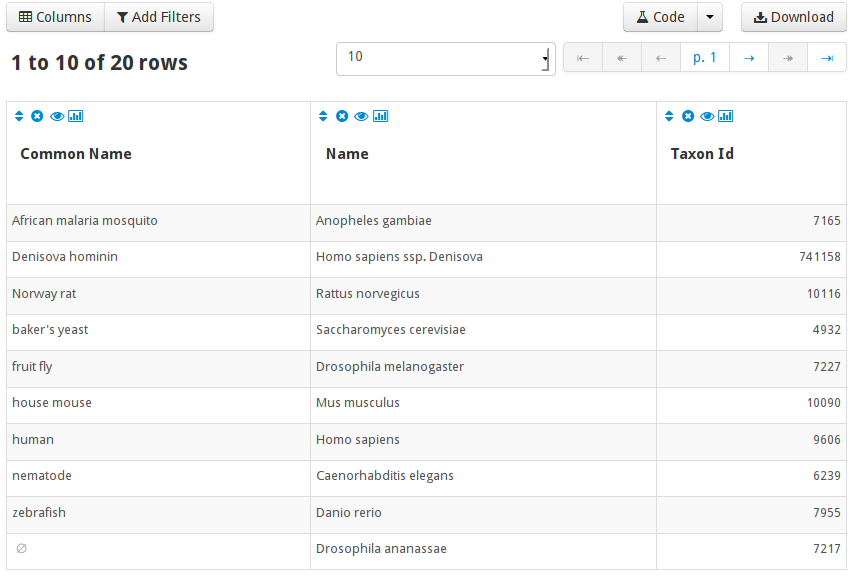
\includegraphics[width=0.4\textwidth]{imtable.png}
\caption{
    \label{fig:1}
    A table of data loaded from FlyMine displaying the output
   of Code Listing ~\ref{code:simple-query}
}
\end{figure}

\begin{figure}
\centering
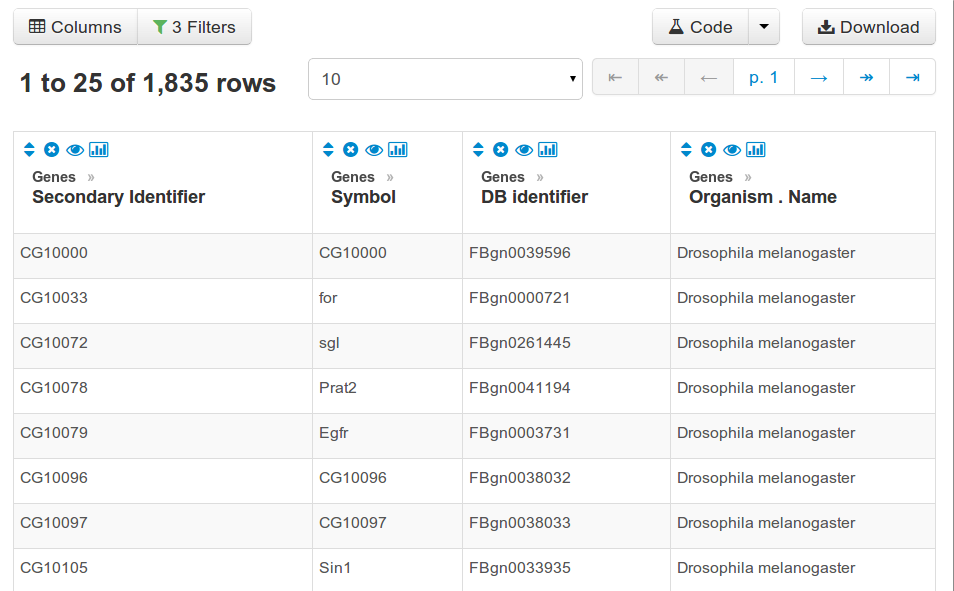
\includegraphics[width=0.4\textwidth]{imtable-complex.png}
\caption{
    \label{fig:complex}
    A table of data loaded from FlyMine displaying the output of Code Listing
    ~\ref{code:complex-query}.
}
\end{figure}

\subsubsection*{Interaction}

The table, as well as providing a number of common dynamic features such as
resorting, pagination and column rearrangement, also permits much deeper
interaction than other comparable table libraries. The table allows the
underlying query to be changed: the constraints of the underlying query can be
edited (Figure ~\ref{fig:edit-filters}); columns (including ones referring to
data types not in the original query) can be added; existing columns can be
removed; changes made can be undone; the data can be exported in a number of
formats or sent to another application, such as a local Galaxy
~\cite{goecks2010galaxy}, ~\cite{blankenberg2010galaxy},
~\cite{giardine2005galaxy} instance, or to a remote application such as
GenomeSpace~\cite{genomespace} (Figure ~\ref{fig:export}); the results can be
saved as a resusable set (a \emph{list}) within the originating service;
individual items can also be previewed (Figure~\ref{fig:preview}).

\begin{figure}[htb]
\centering
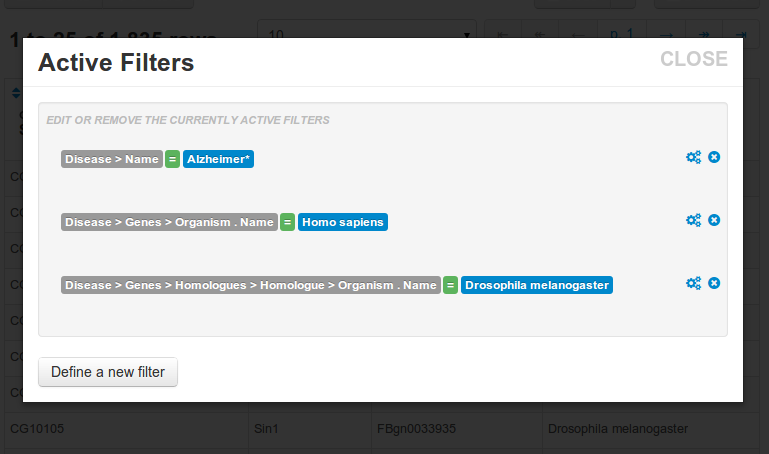
\includegraphics[width=0.4\textwidth]{table-edit-filters.png}
\caption{\label{fig:edit-filters} Editing the filters on a table.}
\end{figure}

\begin{figure}[htb]
\centering
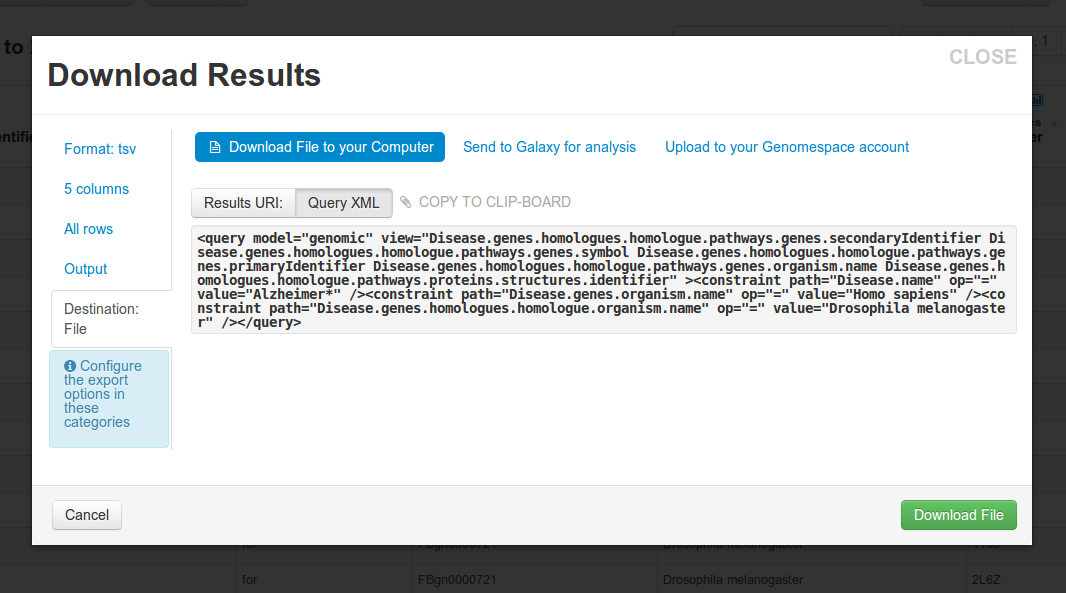
\includegraphics[width=0.4\textwidth]{table-download.png}
\caption{\label{fig:export} Downloading the results of a query.}
\end{figure}

\begin{figure}[htb]
\centering
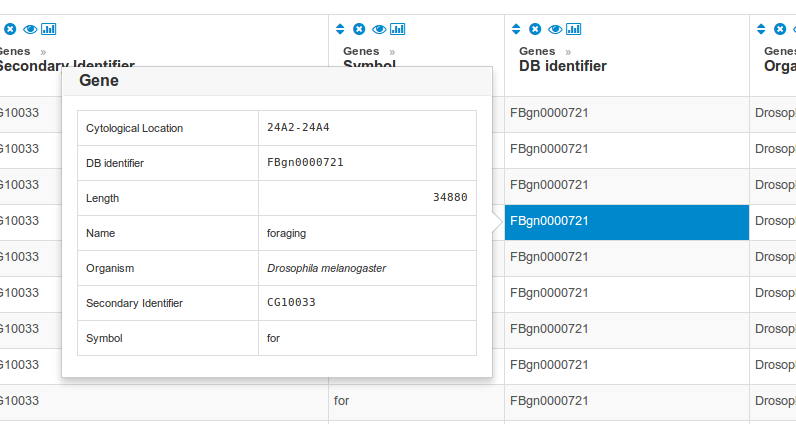
\includegraphics[width=0.4\textwidth]{preview-gene.png}
\caption{\label{fig:preview} Previewing an item.}
\end{figure}

One particularly useful feature is the ability to view the contents of a
single column, analysing it on aggregate and adding or editing filters. This
facility is able to present summary charts for columns based on data type:
binned histograms for numerical data (Figure~\ref{fig:column-summary}), and
column charts for categorical data (Figure~\ref{fig:cat-column-summary},
showing the user adding a filter by selecting items from the column).

\begin{figure}[t]
\centering
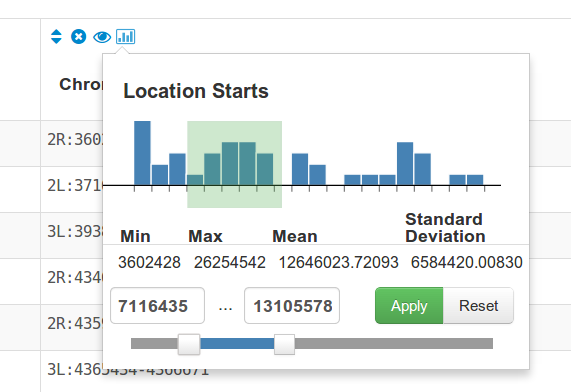
\includegraphics[width=0.4\textwidth]{im-tables-column-summary.png}
\caption{
    \label{fig:column-summary}
    Analysing and filtering a single column of numeric data within a table.
}
\end{figure}

\begin{figure}[t]
\centering
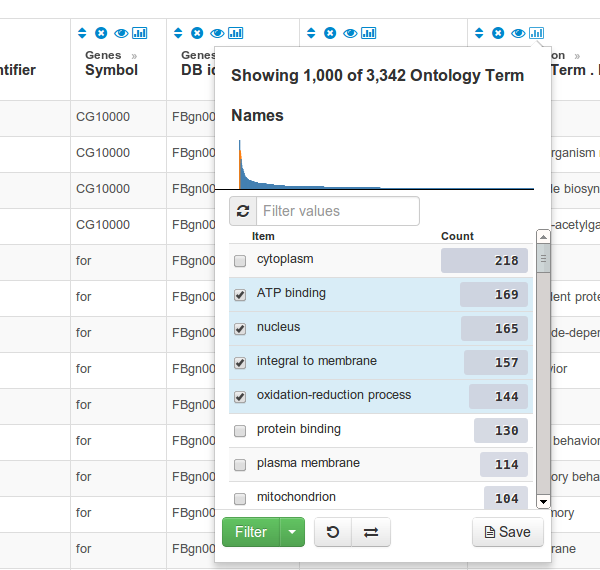
\includegraphics[width=0.4\textwidth]{category-column-summary.png}
\caption{
    \label{fig:cat-column-summary}
    Analysing and filtering a single column of categorical data within a table.
}
\end{figure}

\subsubsection*{Events}

The standard mechanism for communication between components in JavaScript is
event signalling. As per the BioJS specification, this component supports other
objects registering event listeners so they may be notified when events of
interest (such as user interactions) occur.

Once loaded, the table may emit a number of different events (as listed in the
API documentation~\cite{site:biojs-doc}), and may be manipulated by calling 
methods on the instance, allowing the calling page to respond to 
user interactions. For example, if a developer wished to receive notifications 
when the user clicks on any of the cells in the table, they can register to 
listen for these events:

\begin{lstlisting}[caption={Adding an Event Listener}, label={code:add-listener}]
table.addListener("imo:click", function (type, id) {
  alert("User clicked on " + type + " " + id);
});
\end{lstlisting}

This integration means that the table need not be an isolated part of an
application, but can be fully integrated with other components. For example,
instead of just notifying the user by using \emph{alert}, the information about
this object could be displayed in another component. If the user clicked on a
protein, this could be detected, and other suitable components could be
instantiated to display protein-specific analysis (see code
sample~\ref{code:integration}).

\begin{lstlisting}[caption={Integrating with Other Components - Example 1}, label={code:integration}]
table.addListener("imo:click", function (type, id) {
  if ("Protein" === type) {
    table.service.findById(type, id)
                 .then(loadProteinStructureDisplayer);
  }
  function loadProteinStructureDisplayer(protein) {
    // ... load other BioJS component here.
  }
});
\end{lstlisting}

As well as responding to user interaction with the table, the table component
exposes an API to change the state of the table by changing the query it
represents. This allows communication in the other direction. For example if a
linked component, such as a protein structure displayer, emits an event
indicating the user has selected a given set of protein domains, the table could
be modified by adding a filter for these domains to the current query (see code
sample~\ref{code:modify-query}):

\begin{lstlisting}[caption={Integrating with Other Components - Example 2}, label={code:modify-query}]
/* Assuming a "displayer" component that emits the "domains:selected" event */
displayer.addListener("domains:selected", function (domains) {
  var currentQuery = table.getQuery();
  currentQuery.addConstraint({
    "Gene.proteins.proteinDomains.identifier": domains
  });
});
\end{lstlisting}

In this way, the interoperability of these components makes them of increasing
utility to developers, as more of them are published and integrated into third
party applications.

\section*{Discussion}

This tool addresses an important set of needs for bioinformatics developers.
While there are some other libraries that aim to make creating dynamic tables
easy to develop (such as DataTables~\cite{site:datatables}), there are none that
tightly integrate facilities such as query constraint editing, column summary
analysis, data export, support for genomic data types, and list management
without a great deal of development effort. Access to flexible and powerful
data-warehousing tools on the InterMine platform makes these table components
uniquely powerful in the life sciences sphere. Services that implement the
InterMine public API are also able to make use of the features of these tables.
The extremely high quality data sets curated by the principal Model Organism
databases, which the the InterMOD project members make available, makes this
tool unique in its immediate access to integrated life sciences data. 

\section*{Conclusions}

It is hoped that this component will prove useful to those developing tools for
researchers in the life sciences. Various publically funded groups, such as the
MODs and other data-producing consortia, have put significant effort into
creating, curating and composing high quality data sets. InterMine is an
effective platform to add value to this work by integrating the data and
exposing a flexible query API and user interface. The recent work in exposing
these resources through web-services and producing reusable web-based components
allows this investment to benefit not just visitors to the sites of InterMine
applications, but any developer or user who wants to include complex query tools
as part of their platform. With access to a broad range of data sources meeting
the needs of several diverse research communities, we expect that a great deal
of duplicated effort can be avoided, saving significant amounts of time and
money.

\subsection*{Author contributions}
Alex Kalderimis wrote the manuscript and implemented the component, under the
supervision of Gos Micklem, to a set of user specifications supplied by Julie
Sullivan. Rachel Lyne, Radek Štěpán and Mike Lyne contributed to the
component design and revised the manuscript. All authors have approved the
manuscript.

\subsection*{Acknowledgements}
The authors thank Manuel Corpas for useful feedback.

\subsection*{Competing interests}
No competing interests were disclosed.

\subsection*{Grant information}
InterMine has been developed with the support of the following grants, awarded
to Dr. G. Micklem: the Wellcome Trust (Grant number: 090297),
and the National Human Genome Research Institute (Grant number: R01HG004834).

The content is solely the responsibility of the authors and does not necessarily
represent the official views of the funding bodies.

\nocite{*}
{\small\bibliographystyle{unsrt}
\bibliography{references}}

\section*{Supplementary materials}
\appendix
\section{Dependencies} \label{sec:deps}

\lstset{language=HTML}

\begin{lstlisting}
<link
 rel="stylesheet"
 type="text/css"
 href="http://cdn.intermine.org/js/
intermine/im-tables/latest/imtables.css">
<script
 charset="UTF-8"
 type="text/javascript"
 src="http://cdn.intermine.org/js/
intermine/im-tables/latest/imtables-bundled.js">
</script>
\end{lstlisting}

Here we are referring to resources which are made publically available
as part of a Content Delivery Network (CDN). These resources could just
as well be hosted locally.

\end{document}

% vim: textwidth=80 colorcolumn=81
